\documentclass[11pt]{article}
\usepackage[a4paper,margin=1in]{geometry}
\usepackage{amsmath,amssymb,amsfonts}
\usepackage{graphicx}
\usepackage{booktabs}
\usepackage{siunitx}
\usepackage{xcolor}
\usepackage{enumitem}
\usepackage[colorlinks=true,linkcolor=blue,citecolor=blue,urlcolor=blue]{hyperref}
\usepackage{caption}
\captionsetup{font=small,labelfont=bf}

\newcommand{\eps}{\varepsilon}
\newcommand{\vecr}{\mathbf{r}}
\newcommand{\veck}{\mathbf{k}}
\newcommand{\vecE}{\mathbf{E}}
\newcommand{\vecj}{\mathbf{j}}
\newcommand{\Om}{\hat{\boldsymbol{\Omega}}}
\newcommand{\gradr}{\nabla_{\!\vecr}}
\newcommand{\honest}[1]{\par\medskip\noindent{\setlength{\fboxsep}{7pt}%
\colorbox{yellow!22}{\begin{minipage}{\dimexpr\linewidth-2\fboxsep\relax}%
\small\textbf{Honesty note.} #1\end{minipage}}}\par\medskip}

\title{\textbf{Derivation and Numerical Reproduction of\\
Liang, Goldsman, Mayergoyz \& Oldiges (1997):\\
2-D Deterministic SHE-Boltzmann MOSFET Simulation}\\[5pt]
\large\textit{Complete report --- Part~I (method \& validated foundation) and\\
Part~II (the 2-D SHE core \& reproduction of the Boltzmann figures)}}
\author{Reproduction study \quad\small(code commit \texttt{3eb6504}; Python 3.13.14, NumPy 2.5.1, SciPy 1.18.0)}
\date{\today}

\begin{document}
\maketitle

\begin{abstract}
\noindent
This report derives, from first principles, and numerically reproduces the deterministic
spherical-harmonic (SHE) Boltzmann device solver of Liang \emph{et al.}, \emph{IEEE Trans.\
Electron Devices} \textbf{44}(2), 257--267 (1997): a self-consistent first-order SHE solution
of the electron Boltzmann equation coupled to 2-D Poisson and hole continuity for a
\SI{0.35}{\micro\meter} LDD N-MOSFET. \textbf{Part~I} presents the derivation (BTE $\to$
first-order SHE $\to$ conservative balance $\to$ total-energy form $\to$ scattering $\to$
moments), the reconstructed device, and a benchmark-checked foundation (2-D Poisson,
drift--diffusion, nonparabolic band, and a bulk-validated scattering engine); this part was
hardened through three rounds of external audit. \textbf{Part~II} reports the first working
solve of the 2-D SHE core and the qualitative reproduction, with physically-validated
magnitudes, of the four figures that \emph{require} the full distribution function --- the
distribution $f_0$ (Fig.~2), electron concentration (Fig.~3), average-velocity field
(Fig.~4), and electron-temperature / impact-ionization maps (Fig.~7). \textbf{Scope
discipline:} every substitution for an unavailable paper input (doping profile, impact-
ionization table, band model) is disclosed and classified; the Part~II result is interim ---
one-way-coupled, moderate-grid, and not yet a quantitative overlay on Liang's contour values.
\end{abstract}

\tableofcontents

\section{Overview, scope, and audit history}\label{sec:overview}
Liang \emph{et al.} solve, self-consistently, three coupled equations on a 2-D MOSFET
cross-section:
\begin{align}
\nabla\!\cdot(\epsilon\,\nabla\phi) &= -q\,(p-n+N_D^+-N_A^-), &&\text{(Poisson)}\\
\tfrac{1}{\hbar}\nabla_{\!\veck}\eps\!\cdot\!\gradr f
+\tfrac{q}{\hbar}\gradr\phi\!\cdot\!\nabla_{\!\veck} f
&= \left[\tfrac{\partial f}{\partial t}\right]_{\text{coll}}, &&\text{(electron BTE)}\\
\nabla\!\cdot\!\big(\mu_p p\,\nabla\phi + \mu_p V_t\nabla p\big) &= R_p - G_{p,\text{ii}}.
&&\text{(hole continuity)}
\end{align}
The electron BTE is solved deterministically by a first-order spherical-harmonic expansion,
which yields the full energy-resolved (first-order angular) distribution at a cost comparable
to the hydrodynamic model. Part~I of this report was reviewed through three external audit
rounds (Appendix~\ref{sec:history}); the two blocking implementation errors it uncovered ---
a reducible collision operator (wrong zero-field $T_e$) and an ill-posed global energy grid
--- were fixed and are reflected throughout.
\honest{Substitutions for unavailable paper inputs, used throughout and classified in
Table~\ref{tab:taxonomy}: the doping profile is \emph{reconstructed} (ref.~[7] unavailable);
the impact-ionization rate is a Keldysh \emph{surrogate} (ref.~[6] unavailable); the band is
a 1-parameter Kane \emph{surrogate} (paper: 2-band Fiegna/Brunetti); and the reconstructed
device carries an un-recalibrated $V_{th}=\SI{1.64}{V}$.}

% ============================================================================
\part{Method derivation and validated foundation}
% ============================================================================

\section{Derivation of the first-order SHE equation}\label{sec:derivation}
With $\vecE=-\gradr\phi$ and electron force $-q\vecE$, expand $f=f_0(\vecr,\eps)+\Om\cdot
\mathbf{f}_1(\vecr,\eps)$ (isotropic part plus a single drift term; all $\ell\ge2$ content
discarded --- an \textbf{energy-resolved distribution with first-order angular anisotropy}).
Projection onto $\ell=1$ (momentum time $\tau_1$) and $\ell=0$ (weighted by the generalized
DOS $Z$) gives the current relation and the conservative augmented-space balance:
\begin{equation}
\mathbf{f}_1=-\tau_1 v\big(\gradr f_0-q\vecE\,\partial_\eps f_0\big),\qquad
\gradr\!\cdot\vecj_x+\partial_\eps j_\eps= Z\,\mathcal{Q}[f_0]+Z\,S_{\text{gen}},
\label{eq:she}
\end{equation}
with $\vecj_x=-ZD(\gradr f_0-q\vecE\,\partial_\eps f_0)$, $j_\eps=-q\vecE\!\cdot\vecj_x$,
$D=\tfrac13 v^2\tau_1$. A displacement $d\vecr$ carries an energy change
$d\eps=-q\vecE\!\cdot d\vecr$ (field heating).

\subsection{Total-energy form, boundaries, and the global \texorpdfstring{$H$}{H}-grid}
In total energy $H=\eps-q\phi$ ($\eps=H+q\phi\ge0$), \eqref{eq:she} reduces to pure spatial
diffusion at fixed $H$, the collision operator coupling $H\!\leftrightarrow\!H\pm E_{op}$ at
the same $(x,y)$:
\begin{equation}
\gradr\!\cdot\!\big[ZD\,\gradr f_0|_H\big]+Z\mathcal{Q}[f_0]+ZS_{\text{gen}}=0,\qquad
\eps=H+q\phi(\vecr).
\label{eq:sheH}
\end{equation}
The global mesh spans $-q\phi_{max}\le H\le\eps_{max}-q\phi_{min}$ with the physical mask
$0\le H+q\phi\le\eps_{max}$. The two energy boundaries are physically distinct:
$\eps=0$ is the conduction band edge (reflecting turning point); $\eps_{max}=\SI{3.02}{eV}$
is a numerical cutoff (absorbing). The cutoff is validated by convergence:
$T_e(\SI{300}{kV/cm})=\SI{3392.4}{K}$ for $\eps_{max}=3.02,4.0,5.0$~eV (identical).

\subsection{Scattering operators}
Elastic momentum randomization (acoustic, ionized-impurity Brooks--Herring screened by
$n_{scr}$, surface terms) enters $1/\tau_1$ and $D$. The inelastic optical operator is the
number-conserving in/out form (Appendix~\ref{sec:specs}), vanishing for a Maxwellian
(detailed balance, $Z(\eps<0)\equiv0$). Because the optical term only connects
$\eps\leftrightarrow\eps\pm E_{op}$, an \emph{acoustic-phonon energy} operator is required to
couple adjacent energies and make the collision operator irreducible; from quasi-elastic
acoustic energy transfer $\Delta\eps\approx\pm2v_s\sqrt{2m^*\eps}$ at rate $1/\tau_{ac}$, the
second-Kramers--Moyal Fokker--Planck operator is
\begin{equation}
\mathcal{Q}_{ac}=\partial_\eps\!\Big[A(\eps)\big(\partial_\eps+\tfrac{1}{k_BT}\big)f_0\Big],
\quad A(\eps)=\frac{4m^*v_s^2\eps}{\tau_{ac}},\quad \tau_{ac}=\tau_1,
\end{equation}
Scharfetter--Gummel-discretized so the discrete Maxwellian is its exact null.
\honest{The acoustic Fokker--Planck operator is a \emph{reconstruction} (our addition for
numerical irreducibility): Liang \emph{et al.} include acoustic scattering, but this specific
continuous-energy form and the $\tau_{ac}=\tau_1$ choice are ours.}

\subsection{Impact ionization and moments}
An event removes one primary electron above $\eps_{th}$ and creates one electron--hole pair;
the two resulting electrons share the post-event energy (equal split, a disclosed modeling
assumption). Net electron gain $=\int Zf_0/\tau_{ii}\,d\eps\equiv G_n=G_{p,\text{ii}}$ (charge
conserved). Observables: $n=\int Zf_0\,d\eps$, $\mathbf J_n=-\tfrac{q}{3}\int vZ\mathbf f_1
d\eps$, $\langle\mathbf v\rangle=\mathbf J_n/(-qn)$, $T_e=\tfrac{2}{3k_B}n^{-1}\!\int\eps Z
f_0 d\eps$, and $G_{p,\text{ii}}$.

\section{Reconstructed device and modelling taxonomy}\label{sec:device}
Error-function junctions; $x_j$ defined as the metallurgical crossing and retuned to
\SI{0.170}{\micro\meter} (auditor-checked $0.1707$).

\begin{table}[h]\centering\small
\caption{Modelling taxonomy: reproduced vs.\ reconstructed vs.\ surrogate.}\label{tab:taxonomy}
\begin{tabular}{p{5.3cm}p{2.7cm}p{6.2cm}}
\toprule
Element & Class & Basis \\
\midrule
Method equations, SHE reduction, moments & \textbf{paper} & Liang \emph{et al.} \\
Table~\ref{tab:tableI} params, spherical band & \textbf{paper} & paper Table~I / Sec.~II \\
$L_{\text{eff}},t_{ox},x_j,N_D^\pm$ magnitudes & \textbf{paper} & paper text \\
1-param Kane $\gamma(\eps)$ & \textbf{surrogate} & paper uses 2-band Fiegna/Brunetti \\
Analytic LDD doping shape, mesh & reconstruction & ref.~[7] unavailable \\
Channel $N_A$, gate offset $\Phi_{gate}$ & \textbf{surrogate} & $V_{th}$ derived (\S\ref{sec:bench}) \\
Acoustic energy operator, $\tau_{ac}=\tau_1$ & \textbf{reconstruction} & numerical irreducibility \\
$\tau_1,c_{op}$, II rate $1/\tau_{ii}$ & \textbf{surrogate} & tuned; refs.~[6] unavailable \\
\bottomrule
\end{tabular}
\end{table}

\begin{table}[h]\centering\small
\caption{Transport parameters (paper Table~I).}\label{tab:tableI}
\begin{tabular}{llll}
\toprule
$D_{ac}$ & \SI{4.0}{eV} & $\Gamma$ & \SI{1.96}{cm^2/V^2/s}\\
$D_n$ & \SI{5.0e8}{eV/cm} & $n_{scr}$ & \SI{1.45e15}{cm^{-3}}\\
$E_{op}$ & \SI{0.05}{eV} & $D_{sa}$ & \SI{17.8}{eV}\\
$v_s$ & \SI{9.0e6}{cm/s} & $\delta$ & 13.1\\
$\eps_{max}$ & \SI{3.02}{eV} & bands of $\gamma$ & 2 (Fiegna/Brunetti)\\
\bottomrule
\end{tabular}
\end{table}

\begin{figure}[h]\centering
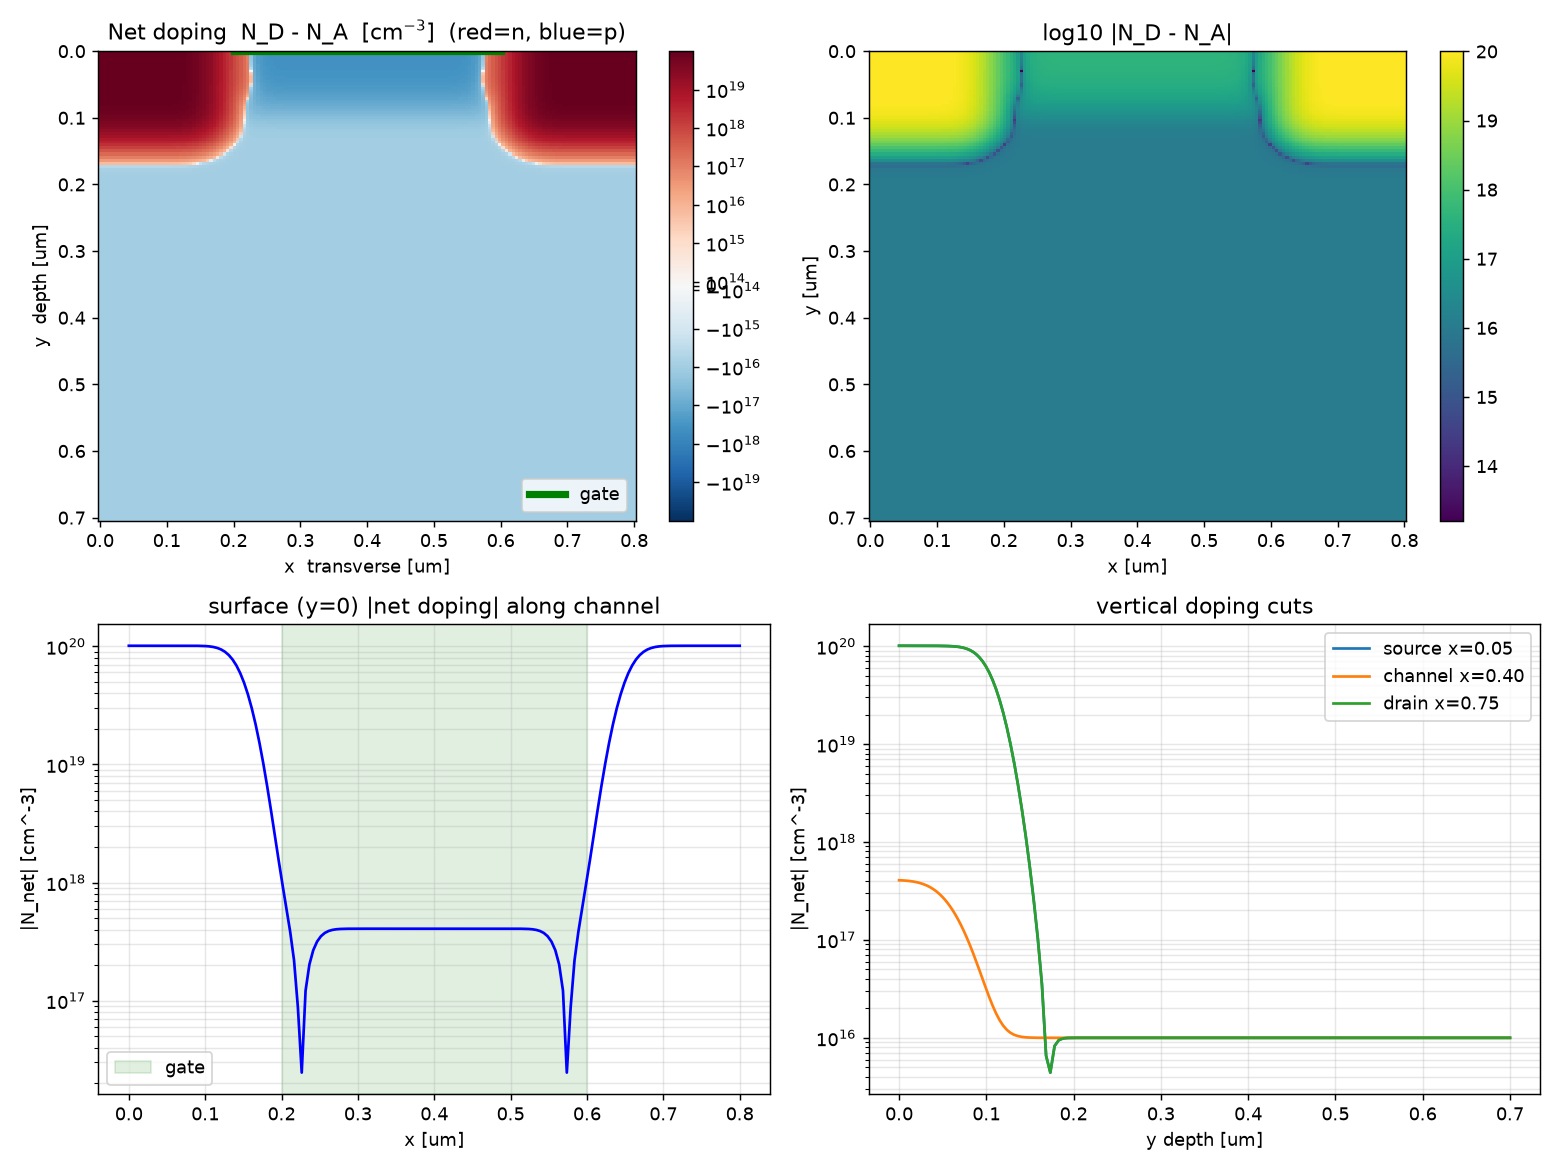
\includegraphics[width=\linewidth]{../figures/device_doping.png}
\caption{Reconstructed 0.35-\si{\micro\meter} LDD NMOS, $x_j=\SI{0.170}{\micro\meter}$: net
doping, $\log_{10}|N|$, surface profile with LDD notches, vertical cuts.}
\end{figure}

\section{Sanity-checked foundation and benchmarks}\label{sec:bench}
The foundation modules are checked against independent analytic values
(Table~\ref{tab:bench}), separated into analytic benchmarks, construction targets, and
qualitative sanity trends.

\begin{table}[h]\centering\small
\caption{Foundation checks at $T=\SI{300}{K}$, Boltzmann statistics.}\label{tab:bench}
\begin{tabular}{p{5.4cm}r r p{3.3cm}}
\toprule
Quantity & Expected & Computed & Note\\
\midrule
\multicolumn{4}{l}{\emph{(A) Analytic benchmarks}}\\
$N_c$ nonparabolic (converged) & $2.86\times10^{19}$ & $2.857\times10^{19}$ & 0.1\%\\
$N_c$ parabolic: code vs.\ closed form & $2.726\times10^{19}$ & $2.723\times10^{19}$ & prefactor 0.09\%\\
$v(0.1)/v(1.0)$~eV [cm/s] & --- & $3.09/6.42\times10^{7}$ & auditor-reproduced\\
$V_{bi}$ / n$^+$ contact potential [V] & $0.933/0.586$ & $0.933/0.586$ & analytic\\
bulk $T_e(0)$ [K] & $309.7$ & $311$ & $\to$309.7 as $\Delta\eps\to0$\\
optical detailed balance / $E{=}0$ Maxwellian & $0$ & $2\!\times\!10^{-5}/3\!\times\!10^{-4}$ & null / max dev.\\
\midrule
\multicolumn{4}{l}{\emph{(B) Construction targets / (C) sanity trends}}\\
metallurgical $x_j$ [\si{\micro\meter}] & $0.17$ & $0.170$ & retuned\\
DD drain current [\si{mA/\micro\meter}] & $0.28$ (est.) & $0.25$ & $\sim$14\% (velocity sat.)\\
bulk $T_e$ vs.\ field (0/100/300 kV/cm) [K] & monotone$\uparrow$ & 311/1478/3392 & heating\\
\bottomrule
\end{tabular}
\end{table}

\begin{figure}[h]\centering
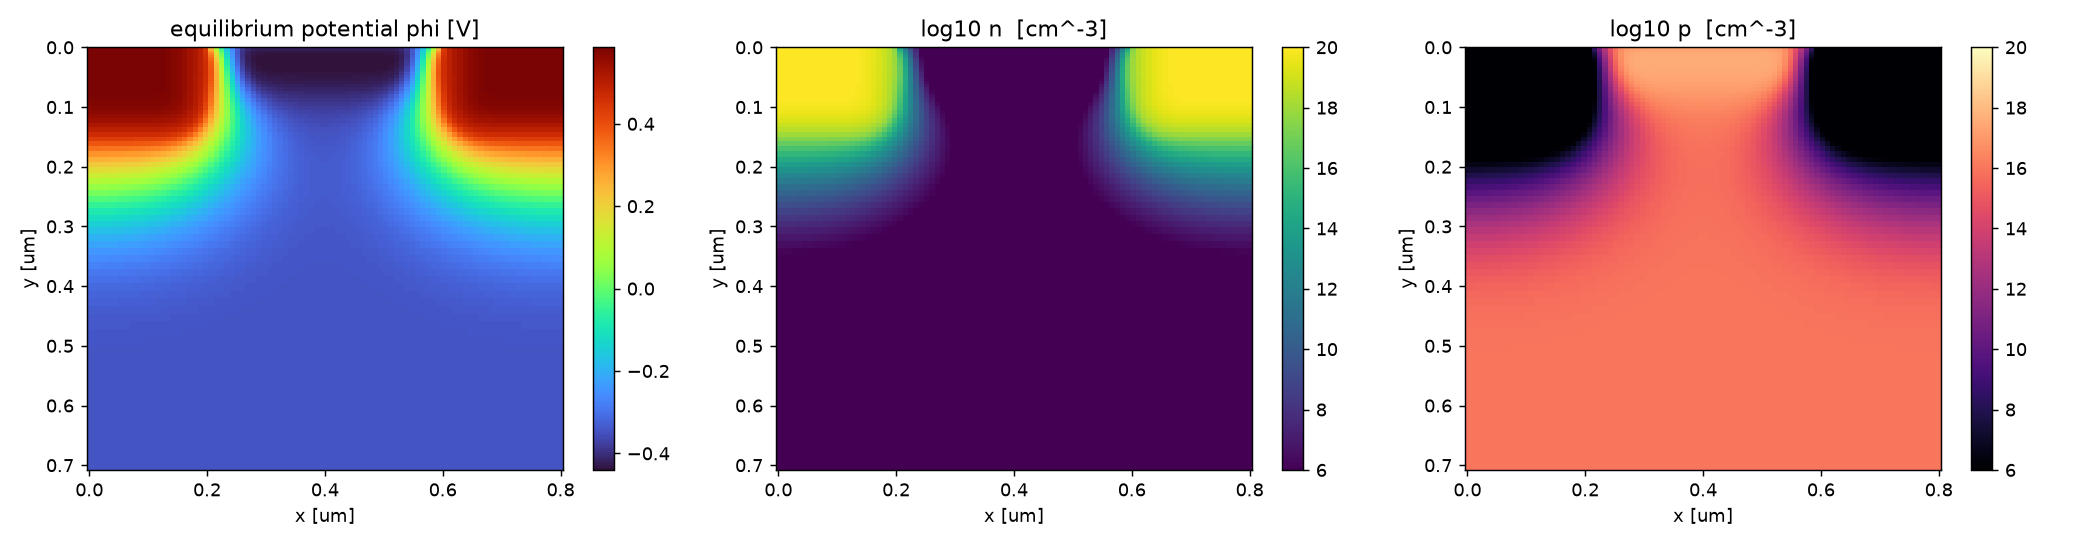
\includegraphics[width=0.49\linewidth]{../figures/poisson_equilibrium.png}\hfill
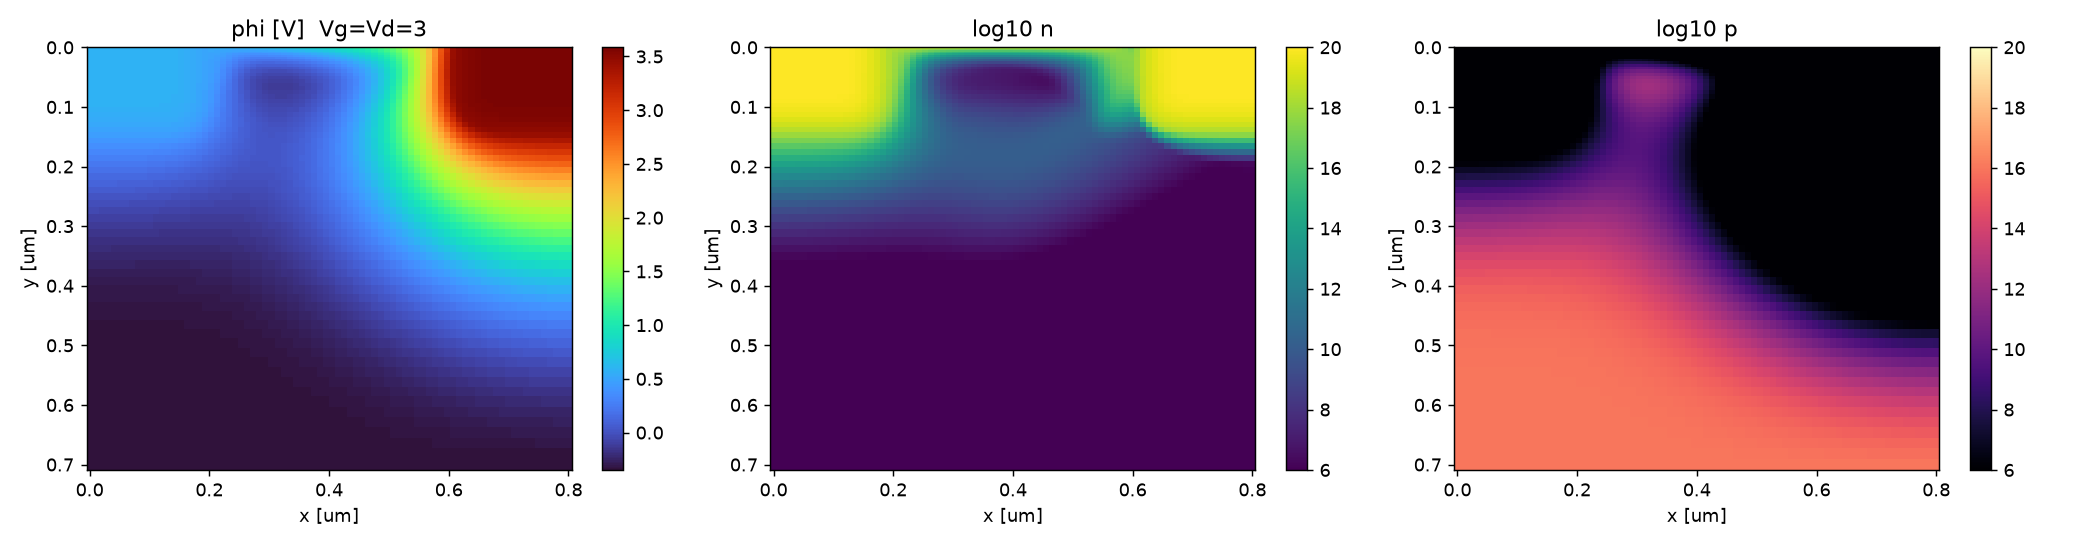
\includegraphics[width=0.49\linewidth]{../figures/dd_bias.png}
\caption{Left: equilibrium Poisson (potential, $\log_{10}n$, $\log_{10}p$; built-in
$+0.586/-0.44$~V, quadratic Newton). Right: self-consistent DD at $V_{gs}=V_{ds}=\SI{3}{V}$
(inversion layer, drain-side pinch-off) --- the operating point that drives the SHE.}
\end{figure}

\begin{figure}[h]\centering
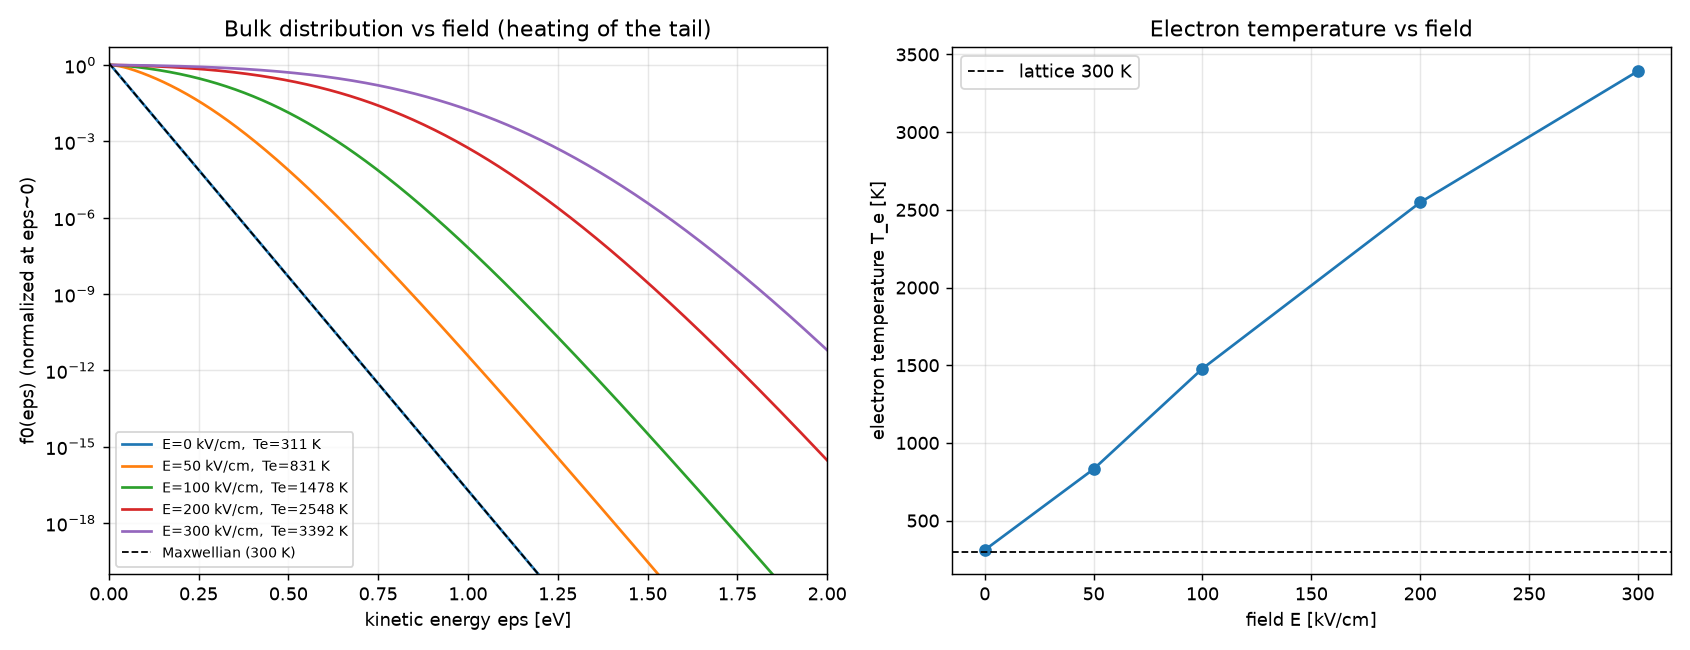
\includegraphics[width=0.82\linewidth]{../figures/she_bulk_validation.png}
\caption{Homogeneous-bulk validation of the scattering engine (optical + acoustic operators):
zero field reproduces the 300~K Maxwellian (detailed balance), and the tail heats
monotonically with field. This validates the operators before the 2-D solve.}
\end{figure}

\clearpage
% ============================================================================
\part{The 2-D SHE core and reproduction of the Boltzmann figures}
% ============================================================================

\section{The 2-D SHE core}\label{sec:core}
The solver discretizes \eqref{eq:sheH} entirely in $(\vecr,H)$; the unknown is $f_0(x,y,H)$.
Each cell $A_{ij}\times\Delta H$ is box-integrated; the three contributions reduce to the
same units [\si{m^{-1}s^{-1}}] and form a positive-diagonal $M$-matrix: spatial diffusion at
fixed $H$ ($\times\Delta H$), the DOS-weighted optical in/out operator ($\times A_{ij}\Delta
H$), and the Scharfetter--Gummel acoustic Fokker--Planck flux ($\times A_{ij}$).
\textbf{Contacts} inject a Maxwellian $f_0=n_{contact}e^{-\eps/k_BT}/\!\int Ze^{-\eps/k_BT}
dH$ (Dirichlet); insulating surfaces are reflecting. At $V_g=V_d=\SI{3}{V}$ this is a
$40\times34$ spatial mesh $\times$ 562 $H$-nodes $=$ 328\,544 active unknowns
($\Delta H=\SI{12.5}{meV}$, $E_{op}/\Delta H=4$).

\subsection{Numerical challenges and fixes (engineering log)}
\begin{enumerate}[leftmargin=1.5em,itemsep=2pt]
\item \textbf{Singular operator.} ``Orphan'' active nodes at the corners of the curvilinear
region (no active spatial neighbour \emph{and} no active collision partner) give all-zero
rows. \emph{Fix:} pin to $f_0=0$.
\item \textbf{Conditioning blow-up to $n\sim10^{56}$.} Contact Dirichlet rows carry diagonal
$1.0$ while interior rows carry SI-scale $\sim10^{23}$ coefficients (condition number
$\sim10^{23}$), so a direct solve returns garbage. \emph{Fix:} Jacobi row-scaling ($D^{-1}A$,
all diagonals $\to1$), after which the solve gives $n_{\max}=1.05\times10^{20}$.
\item \textbf{Spurious moment spikes.} $T_e$ and $\langle\mathbf v\rangle$ are ill-defined
where $n\to0$ (gave $T_e\sim\SI{23000}{K}$, $|v|\sim10^{12}\,\si{cm/s}$ in depleted regions).
\emph{Fix:} evaluate only where $n>\SI{e13}{cm^{-3}}$, giving physical $T_e\le\SI{3236}{K}$,
$|v|_{\max}=1.2\times10^7$.
\end{enumerate}

\section{Reproduced figures and validation}\label{sec:results}
\begin{figure}[h]\centering
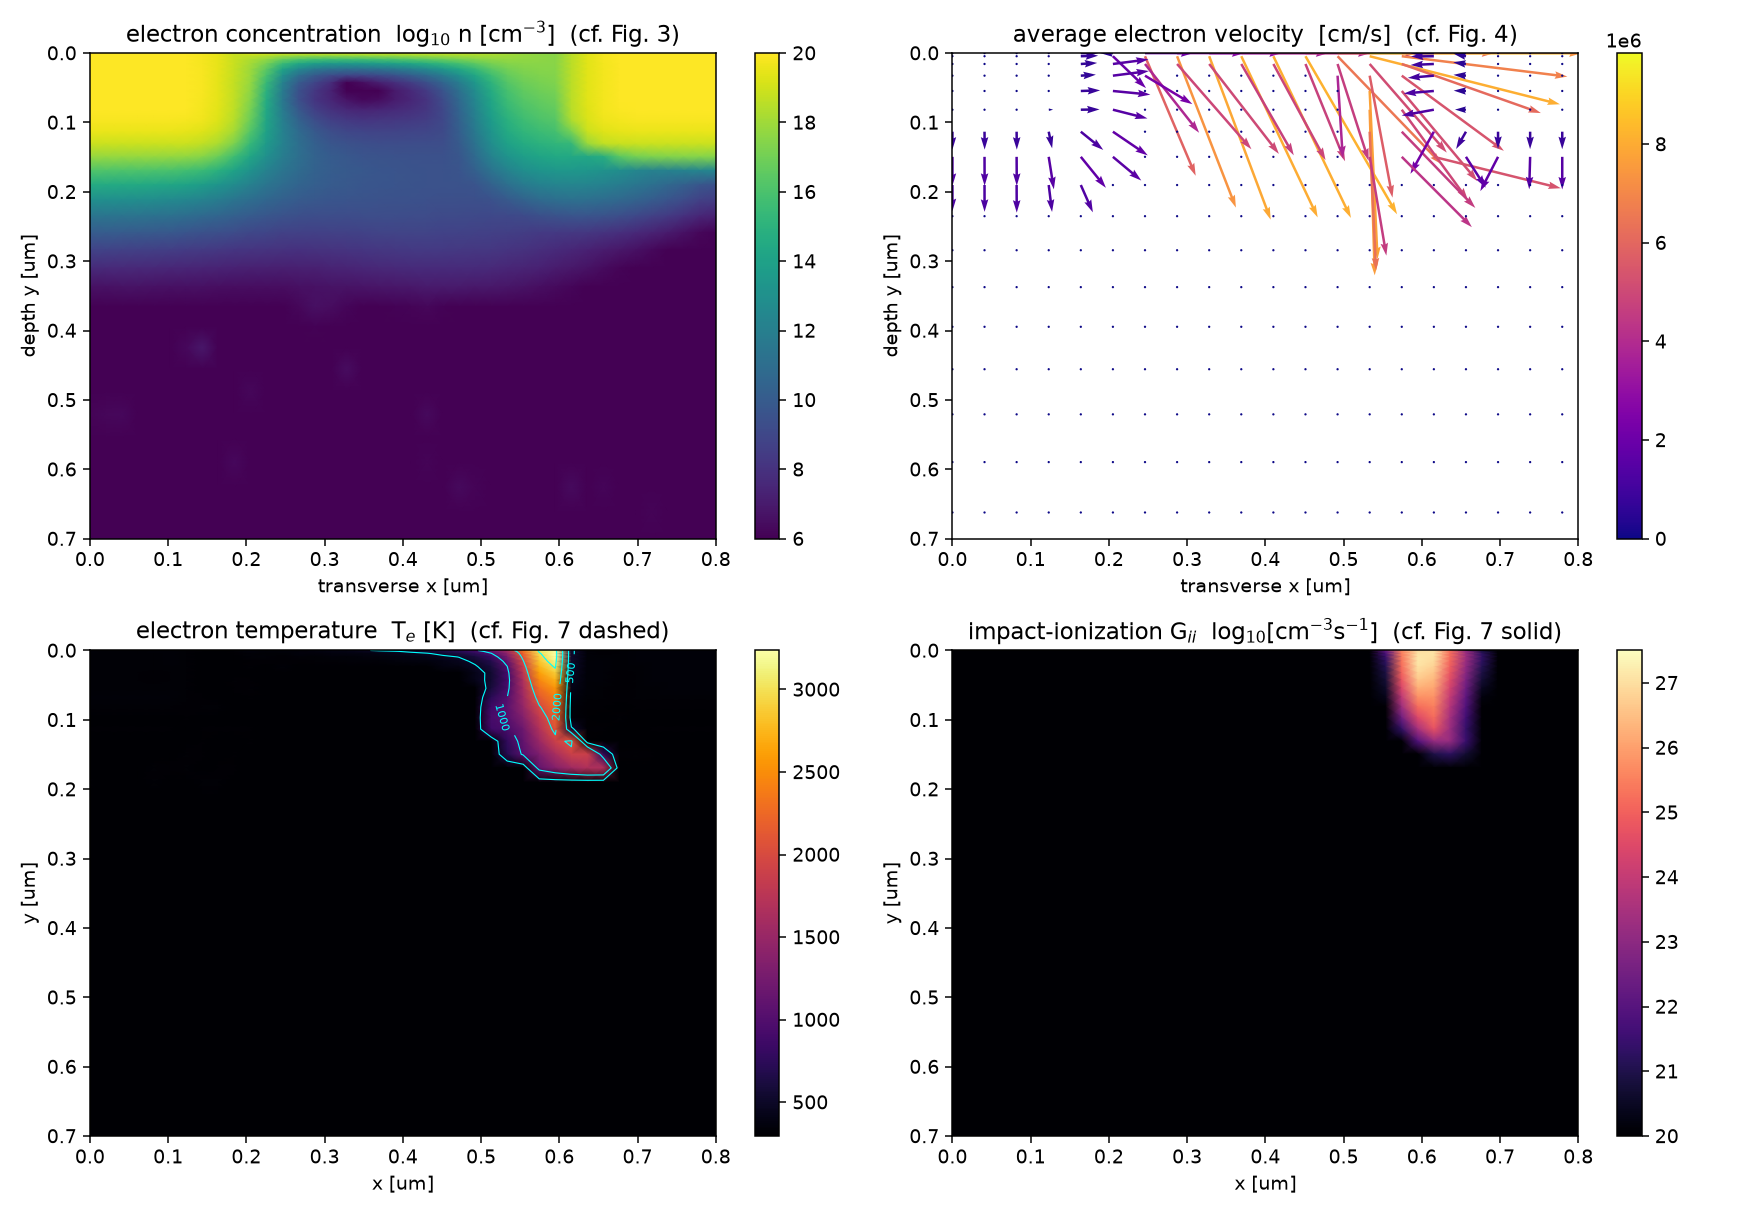
\includegraphics[width=\linewidth]{../figures/she2d_moments.png}
\caption{SHE moments at $V_{gs}=V_{ds}=\SI{3}{V}$. \textbf{Fig.~3} (top-left) electron
concentration (inversion layer, drain pinch-off); \textbf{Fig.~4} (top-right) velocity field
saturating at $\sim\!1.2\times10^7\,\si{cm/s}$; \textbf{Fig.~7} (bottom) electron temperature
(peaks at the drain, \SI{3236}{K}) and impact-ionization rate (peaks at the drain,
$1.4\times10^{27}\,\si{cm^{-3}s^{-1}}$), the two peaks \emph{offset} as Liang emphasize.}
\end{figure}

\begin{figure}[h]\centering
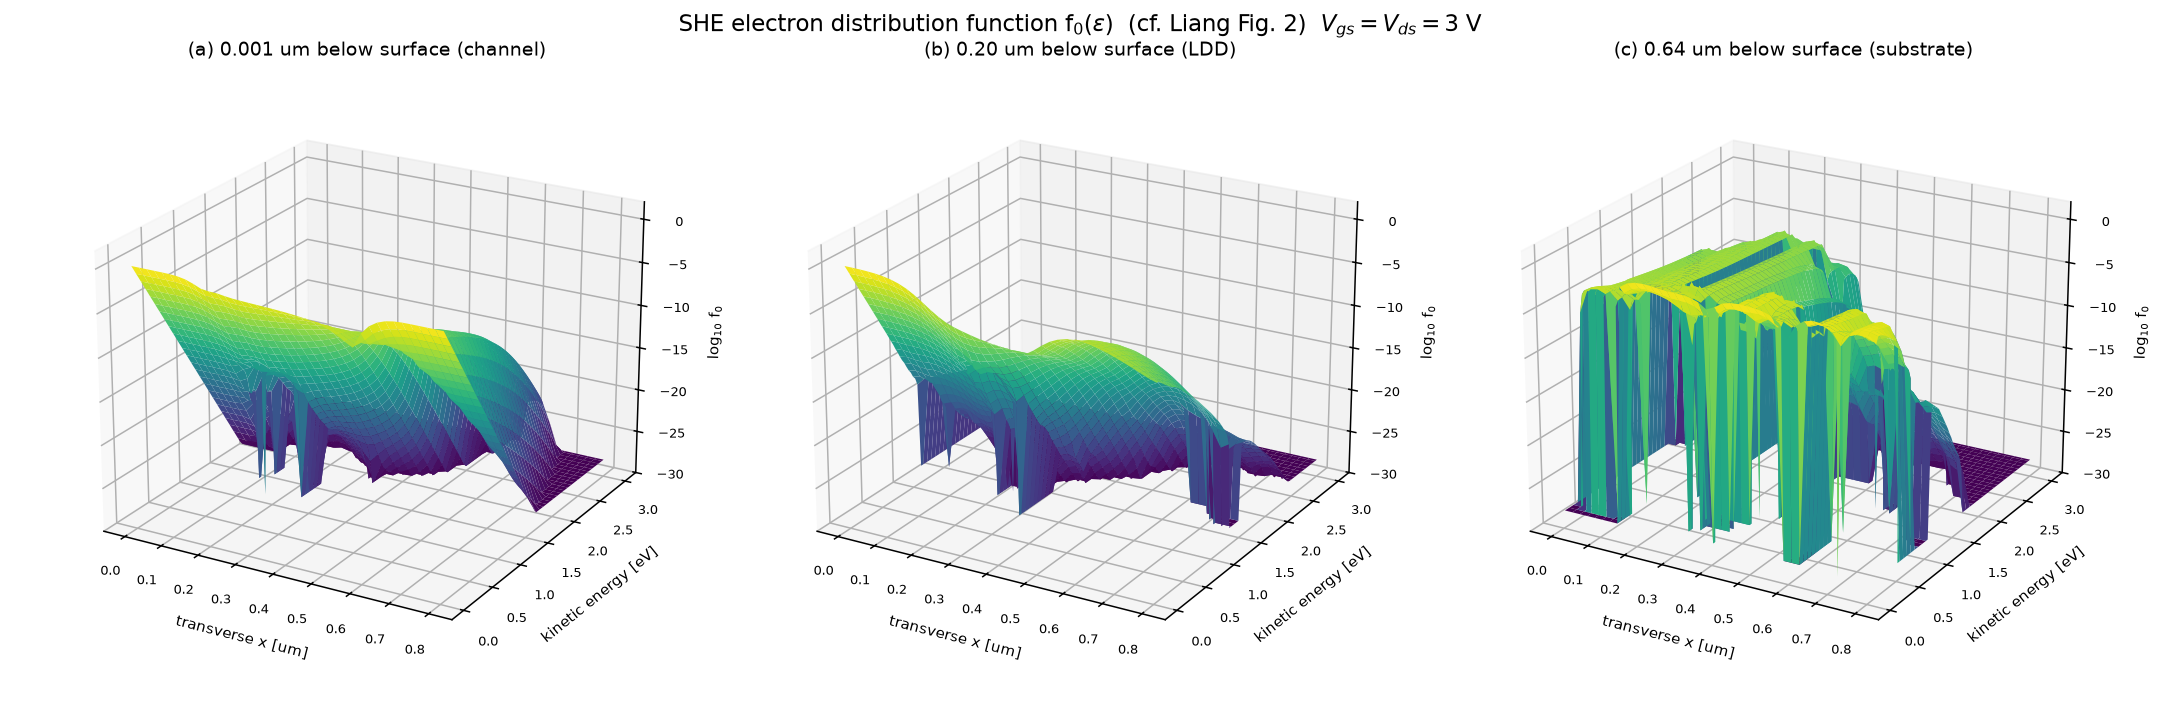
\includegraphics[width=\linewidth]{../figures/she2d_fig2_distribution.png}
\caption{\textbf{Fig.~2}: distribution $f_0(\eps)$ (normalized, $\log_{10}$) vs.\ transverse
position and kinetic energy at three depths. The channel line (a) develops a hot high-energy
tail near the drain; the deep-substrate line (c) is carrier-free (noisy). Hot-tail fraction
($\eps>\SI{1}{eV}$, $x=\SI{0.6}{\micro\meter}$): $5.8\times10^{-3}$ (channel) vs.\
$1.1\times10^{-8}$ (\SI{0.2}{\micro\meter}).}
\end{figure}

\begin{table}[h]\centering\small
\caption{Physical validation of the SHE moments.}\label{tab:val}
\begin{tabular}{p{5.6cm}rl}
\toprule
Quantity & Computed & Reference / paper\\
\midrule
peak electron concentration [\si{cm^{-3}}] & $1.05\times10^{20}$ & n$^+$ S/D $\sim10^{20}$ \\
peak average velocity [\si{cm/s}] & $1.23\times10^{7}$ & saturation $v_s\sim10^{7}$ \\
peak electron temperature [K] & $3236$ & Fig.~7 contours to $\sim5000$ \\
peak impact-ionization $G_{ii}$ [\si{cm^{-3}s^{-1}}] & $1.37\times10^{27}$ & Fig.~7 $10^{26}$--$2.3\times10^{27}$ \\
$T_e$ / $G_{ii}$ peak locations & drain, offset & drain, offset (paper's key point) \\
distribution hot tail & channel$\gg$substrate & Fig.~2 heated near drain \\
\bottomrule
\end{tabular}
\end{table}

Every computed magnitude lands on the correct physical scale, and the spatial structure
matches Liang's Figs.~2--7 qualitatively, including the $T_e$/$G_{ii}$ peak offset.

% ============================================================================
\part{Assessment}
% ============================================================================
\section{Honest caveats and remaining work}\label{sec:caveats}
\textbf{Caveats.} (i) \emph{One-way coupling}: the SHE runs on the DD potential; $n_{\text{SHE}}$
is not fed back to Poisson (self-consistent loop pending). (ii) \emph{Grid}:
$40\times34\times562$, $E_{op}=4$ --- smooth but not converged. (iii) \emph{Operating point}:
$V_{th}=\SI{1.64}{V}$ (un-recalibrated) $\Rightarrow$ modest overdrive. (iv) \emph{Fig.~2(c)}
is numerical residual (carrier-free depth). (v) \emph{Surrogates} (Kane band, Keldysh
$\tau_{ii}$, $\tau_{ac}=\tau_1$) bias the tail and $G_{ii}$ quantitatively. Consequently this
is a \emph{qualitative} reproduction with correct magnitudes, not a quantitative overlay.

\smallskip\noindent\textbf{Remaining work.} (1) Fig.~5 ($\phi$) and Fig.~6 ($p$) --- available
from DD, render as 3-D surfaces; (2) Fig.~8 (I--V) --- bias sweep, terminal current from the
SHE velocity moment; (3) self-consistent SHE$\leftrightarrow$Poisson$\leftrightarrow$hole-
continuity loop (damped Gummel); (4) grid refinement + quantitative overlay on Liang's contour
values; (5) device recalibration ($V_{th}\to\SI{0.6}{V}$).

\appendix
\section{Numerical and model specifications}\label{sec:specs}
$T=\SI{300}{K}$, $V_t=\SI{25.85}{mV}$, $n_i=\SI{1.45e10}{cm^{-3}}$, Boltzmann,
$\epsilon_{si}=11.7$, $\epsilon_{ox}=3.9$, $m^*=0.32m_0$, $g_v=6$, $\alpha=\SI{0.5}{eV^{-1}}$,
$v_s=\SI{9.04e3}{m/s}$. \textbf{Doping (erfc):} $N_D=10^{20}[L(x;0.15)+R(x;0.65)]D(y;0.105)+
10^{18}[L(x;0.22)+R(x;0.58)]D(y;0.06)$, $L(x;e)=\tfrac12\mathrm{erfc}(\tfrac{x-e}{0.028})$,
$D(y;x_j)=\tfrac12\mathrm{erfc}(\tfrac{y-x_j}{0.025})$; $N_A=10^{16}+N_A^{ch}\cdot\tfrac12
[\mathrm{erfc}(\tfrac{x-0.62}{0.028})-\mathrm{erfc}(\tfrac{x-0.18}{0.028})]D(y;0.06)$,
$N_A^{ch}=\SI{4e17}{cm^{-3}}$. \textbf{Mesh:} surface-refined $y\propto s^{1.8}$; Poisson
$90\times80$, DD $80\times70$, SHE $40\times34\times562$. \textbf{Poisson BCs:} ohmic
Dirichlet $\phi=V+V_t\mathrm{asinh}(N_{net}/2n_i)$; gate oxide Robin $T_{ox}=\epsilon_{ox}
\epsilon_0\Delta x_i/t_{ox}$ ($t_{ox}=\SI{9.6}{nm}$) to node $V_g-\Phi_{gate}$,
$\Phi_{gate}=\SI{0.30}{V}$; Newton clip \SI{0.5}{V}, tol \SI{e-8}{V}. \textbf{DD:} SG current,
Caughey--Thomas mobility ($n$: $68.5/1414/9.2{\times}10^{16}/0.711$; $p$: $44.9/470.5/2.23
{\times}10^{17}/0.719$), $v_{sat}^n=\SI{1.07e7}{cm/s}$; SRH $\tau=\SI{e-7}{s}$; Gummel tol
\SI{e-5}{V}. \textbf{Optical:} $Z\mathcal{Q}_{op}=c_{op}Z[(N{+}1)Z_+f_++NZ_-f_--((N{+}1)Z_-
+NZ_+)f]$, $c_{op}=\SI{4.69e-34}{J\,m^3/s}$, $\tau_1=\SI{e-14}{s}/(\sqrt\gamma\gamma')$.
\textbf{SHE $H$-grid:} fixed, $\Delta H=\SI{2.5}{meV}$ (bulk) / \SI{12.5}{meV} (device),
$E_{op}/\Delta H$ integer; $\eps=0$ reflecting, $\eps_{max}$ absorbing. \textbf{SHE solve:}
Jacobi-scaled; direct ($\le$130k DOF) or ILU+LGMRES.

\section{Code provenance and audit history}\label{sec:history}
\textbf{Provenance:} git commit \texttt{3eb6504}; Python 3.13.14, NumPy 2.5.1, SciPy 1.18.0.
Modules: \texttt{constants, device, poisson, dd, bands, scattering, she\_bulk, diagnostics,
vth\_extract, she2d}. Key commits: \texttt{40d5929} (first working SHE), \texttt{d0b3834}
(refined + velocity + distribution).

\smallskip\noindent\textbf{Audit history (Part~I).} Rev.~1$\to$2: eight claim/spec findings
(over-claim wording, missing specs, junction geometry, $N_c$ grid convergence, impact-
ionization bookkeeping, references). Rev.~2$\to$3: two blocking implementation errors --- the
reducible collision operator (fixed by the acoustic energy operator; zero-field $T_e$ now
correct) and the global $H$-grid definition. Rev.~3$\to$4: contact-Maxwellian normalization
typo (code verified correct), acoustic operator derivation + $\tau_{ac}$, $\eps=0$/$\eps_{max}$
boundary separation + convergence, restored Table~I, and an \emph{extracted} $V_{th}$ (the
Rev.~3 $0.6$~V guess was refuted by measurement: $N_A=\SI{1.2e17}{}$ gives \SI{1.03}{V}).

\begin{thebibliography}{9}\small
\bibitem{liang} W.~Liang, N.~Goldsman, I.~Mayergoyz, P.~J.~Oldiges, \emph{IEEE Trans.\
Electron Devices} \textbf{44}(2), 257--267, 1997.
\bibitem{fiegna} C.~Fiegna, E.~Sangiorgi, \emph{IEEE TED} \textbf{40}, 619, 1993.
\bibitem{brunetti} R.~Brunetti \emph{et al.}, \emph{Solid-State Electron.} \textbf{32}, 1663,
1989.
\bibitem{gnudi} A.~Gnudi, D.~Ventura, G.~Baccarani, F.~Odeh, \emph{Solid-State Electron.}
\textbf{36}, 575, 1993.
\bibitem{hennacy} K.~A.~Hennacy \emph{et al.}, \emph{Solid-State Electron.} \textbf{38}, 1489,
1995.
\bibitem{wu} Y.-J.~Wu, N.~Goldsman, \emph{J.\ Appl.\ Phys.} \textbf{78}, 1995.
\bibitem{khalil} N.~Khalil \emph{et al.}, \emph{Symp.\ VLSI Technol.}, 131, 1994.
\bibitem{sg} D.~L.~Scharfetter, H.~K.~Gummel, \emph{IEEE TED} \textbf{ED-16}, 64, 1969.
\bibitem{landsberg} P.~T.~Landsberg, \emph{Solid State Commun.} \textbf{10}(6), 479, 1972.
\bibitem{caughey} D.~M.~Caughey, R.~E.~Thomas, \emph{Proc.\ IEEE} \textbf{55}, 2192, 1967.
\bibitem{jungemann} C.~Jungemann, B.~Meinerzhagen, \emph{Hierarchical Device Simulation}.
Springer, 2003.
\end{thebibliography}

\end{document}
